\documentclass[../sparc.tex]{subfiles}
\graphicspath{{\subfix{../images/}}}
\begin{document}

\section{Звук}
\index{Музыка!Частота звука}
\newglossaryentry{Гц}{name=Гц, description={Герц}}
\newglossaryentry{КГц}{name=КГц, description={Килогерц ($10^3$ Гц)}}
\newglossaryentry{МГц}{name=МГц, description={Мегагерц ($10^6$ Гц)}}
\newglossaryentry{ГГц}{name=ГГц, description={Гигагерц ($10^9$ Гц)}}


Как известно, \emph{звук} -- это колебания (вид сигнала), и каждому
определённому звуку соответствует своя частота колебаний.

Частоты измеряются в \emph{Герцах} (\gls{Гц}), и один Герц (1 Гц) означает одно
колебание в секунду. 10 колебаний в секунду -- 10 Гц, 100 колебаний в секунду --
100 Гц и т. д. Если же мы говорим про частоты в 100 Гц и более, то удобнее
использовать приставки Кило- (\gls{КГц}), Мега- (\gls{МГц}) и Гига- (\gls{ГГц}):
сигнал с частотой 1 КГц поданный на цифровой порт колеблет мембрану динамика
1000 раз в секунду.  Ниже приведена таблица некоторых кратных единиц частот в
Герцах:

\begin{tabular}{p{3cm}|p{4cm}|p{3.5cm}}
  Название & Величина & Пример \\
  \hline \hline
  Герц (Гц)
  & $ 1 \mbox{Гц} $ или $ 10^0 \mbox{Гц} $
  & $ 100 * 10^0 \mbox{Гц} = 100 \mbox{Гц} $ \\
  \hline
  Килогерц (КГц)
  & $ 1000 \mbox{Гц} $ или $ 10^3 \mbox{Гц} $
  & $ 100 * 10^3 \mbox{Гц} = 100 \mbox{КГц} $ \\
  \hline
  Мегагерц (МГц)
  & $ 1000000 \mbox{Гц} $ или $ 10^6 \mbox{Гц} $
  & $ 100 * 10^6 \mbox{Гц} = 100 \mbox{МГц} $ \\
  \hline
  Гигагерц (ГГц)
  & $ 1000000000 \mbox{Гц} $ или $ 10^9 \mbox{Гц} $
  & $ 100 * 10^9 \mbox{Гц} = 100 \mbox{ГГц} $ \\
\end{tabular}

Таким образом, для генерации сигнала нам необходимо знать его частоту в Герцах,
либо знать длину волны.

Зная период, мы можем узнать частоту, и наоборот -- поскольку частота является
ничем иным, как количеством повторений заданных колебаний в секунду. Это удобно
представить визуально (\ref{fig:sound-fig-1}.)

\begin{figure}[h]
  \caption{Визуальное представление частоты колебаний 5 Гц.}
  \label{fig:sound-fig-1}
  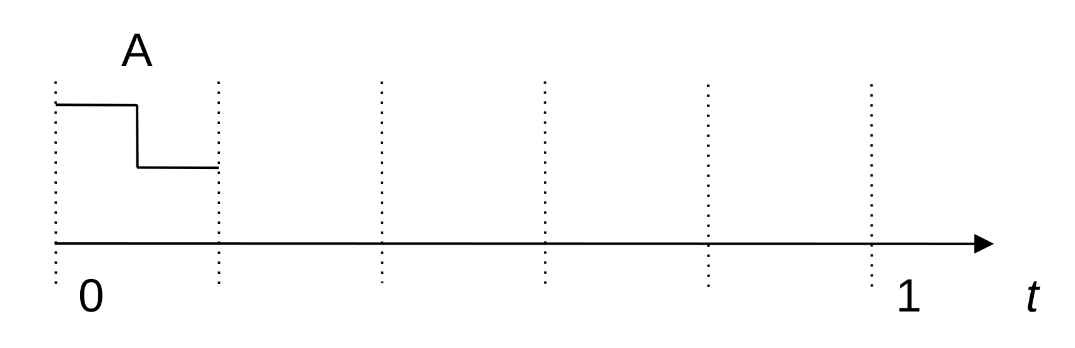
\includegraphics[width=10cm]{sound-fig-1}
  \centering
\end{figure}

Если известно, что колебание А помещается 5 раз в 1 секунду, то говорят, что
частота данного сигнала равна 5 Гц. Узнать период можно, разделив 1 секунду
(заданную в микросекундах) на частоту (5 Гц):

\begin{equation}
  \frac{1000000 \mbox{мкс}}{5 \mbox{Гц}} = 200000 \mbox{мкс}
\end{equation}

Получается, что длина волны равна 200000 мкс, или $ 200 * 10^3 \mbox{мс} $. Если
же нам известна длина волны и нужно узнать частоту, то необходимо разделить 1
секунду (в микросекундах) на длину волны -- таким образом, получим частоту в
Герцах. Всё просто.

Метод генерации звука похож на \gls{ШИМ}. Основные отличия заключаются в том,
что теперь мы должны изменять длину волны \texttt{len}, оставляя коэффициент
заполнения неизменным -- он описывается константой \texttt{DC} и всегда равен
0.5. Поскольку коэффициент заполнения всегда равен 50\% (0.5), то время подачи
сигналов \texttt{HIGH} и \texttt{LOW} всегда одинаково -- иными словами, нам
достаточно вычислить только задержку \texttt{d1}. Это показано на графике ниже:

Как и в случае с ШИМ, начнём писать функцию, которая будет реализовывать
вышеописанные принципы. Функция будет называться \texttt{play\_tone} и будет
позволять генерировать звук с нужной частотой на указанном цифровом порту.

Посмотрим, что данная функция должна принимать в качестве параметров:
\begin{enumerate}
\item Номер цифрового порта, к которому подключен динамик и куда будет
  выводиться звук; назовём этот параметр ``port'';
\item Частота ``f'', измеряемая в Герцах. 
\item Длина звукового сигнала; назовём этот параметр ``t''.
\end{enumerate}

На языке C++ это будет выглядеть примерно так:
\begin{minted}{cpp}
void play_tone(int port, float f, long t) {
    // тело функции
}
\end{minted}

Первым делом в теле функции из частоты найдём период \texttt{T}:
\begin{minted}{cpp}
const long T = 1000000 / f;
\end{minted}

Далее посчитаем длину задержки \texttt{d} -- для этого мы должны поделить период
на 2, то есть, найти \emph{полупериод}:
\begin{minted}{cpp}
long d = T / 2;
\end{minted}

И посчитаем, сколько раз нам нужно повторить период длиной \texttt{p}
микросекунд, чтобы заполнить время \texttt{t}:
\begin{minted}{cpp}
int count = t / T;
\end{minted}

Почти всё готово. Осталось только написать цикл, который будет генерировать
заданную волну нужное количество раз. Здесь отлично подойдёт цикл со счётчиком
(\texttt{for}):

\begin{listing}[H]
  \begin{minted}{cpp}
    for (int i = 0; i < count; i++) {
      digitalWrite(port, HIGH);
      delayMicroseconds(d);
      digitalWrite(port, LOW);
      delayMicroseconds(d);
    }
  \end{minted}
  \label{listing:play-tone-cycle}
  \caption{Реализация цикла генерации звукового сигнала на цифровом порту,
    создающей \texttt{count} колебаний на порту \texttt{port} c полупериодом
    \texttt{d}.}
\end{listing}

В общем виде, функция выглядит так:

\begin{listing}[H]
  \begin{minted}{cpp}
    void play_tone(int port, float f, long t) {
      const long T = 1000000 / f;
      long d = T / 2;
      int count = t / T;
      for (int i = 0; i < count; i++) {
        digitalWrite(port, HIGH);
        delayMicroseconds(d);
        digitalWrite(port, LOW);
        delayMicroseconds(d);
      }
    }
  \end{minted}
  \label{listing:play-tone-procedure}
  \caption{Реализация простой процедуры генерации звукового сигнала на цифровом
    порту.}
\end{listing}

Наша функция генерации звука завершена. Теперь нам нужно подключить динамик к
Arduino и протестировать нашу систему.

\note{Во многих случаях одна и та же задача может быть решена несколькими
  способами.  К примеру, функция \texttt{play\_tone} может быть реализована
  иначе; предложенная нами реализация является только одной из корректных.}

\end{document}
